\chapter{Lecture 9 - Manuel Araújo}

\section{Feynman Integrals - Part 2}

% ── Groupoid of graphs ────────────────────────────────────────────────
\subsection{Groupoid of graphs with prescribed vertices}

Let $V_d$ be the set of vertices with valency $d \in \Zbb_{>0}$.
The groupoid $\mathrm{Graphs}_{V_1, \dots, V_D}$ consists of the data:
\begin{itemize}
  \item \textbf{objects:} matchings in HE (set of half-edges);
  \item \textbf{isomorphisms:} collections of morphisms
    \begin{equation*}
      \varphi_d \colon V_d \longrightarrow V_d, \qquad 0 \leq d \leq D
    \end{equation*}
    and $\varphi \colon HE \to HE$ respecting the incidence maps.
\end{itemize}

The action of the group
\begin{equation*}
  G = \prod_{d = 0}^D
  \underbrace{(S_d)^{V_d}}_{\substack{
      \text{permute} \\ \text{half-edges}
  }} \ltimes 
  \underbrace{S_{V_d}}_{\substack{
      \text{permute} \\ \text{vertices}
  }}
\end{equation*}
on $\text{Matchings}_{2m}$ is such that
\begin{equation*}
  \Stab_\sigma \cong \Aut \Gamma_\sigma, \qquad \forall \sigma \in \lbigslant{G}{\text{Matchings}_{2m}}
\end{equation*}
where $\Gamma_\sigma$ is the graph corresponding to a matching $\sigma$, in the obvious way.
Fixing $g \in G$ and $\sigma \in \Mrm_{2m}$ defines a \textit{canonical} isomorphism
\begin{equation*}
  \Gamma_\sigma \longrightarrow \Gamma_{g \cdot \sigma}
\end{equation*}
and we identify $\mathsf{Graphs}_{V_0, \dots, V_D}$ with the \textit{action groupoid} of $G$ acting on $\text{Matchings}_{2m}$.

\begin{example}
  There is an isomorphism of graphs
  \begin{equation*}
    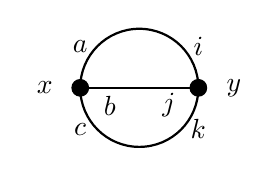
\begin{tikzpicture}[scale = 1.5, baseline=-1mm]
      % lines
      \draw[thick] (0, 0) node at (-.3, 0) {$x$} -- (1, 0) node at (1.3, 0) {$y$};
      \draw[thick] (0, 0) arc (180:0:.5);
      \draw[thick] (0, 0) arc (-180:0:.5);
      % nodes
      \draw[fill=black] (0, 0) circle (2pt);
      \draw[fill=black] (1, 0) circle (2pt);
      \node at (0, .35) {$a$};
      \node at (.25, -.15) {$b$};
      \node at (0, -.35) {$c$};
      \node at (1, .35) {$i$};
      \node at (0.75, -.15) {$j$};
      \node at (1, -.35) {$k$};
    \end{tikzpicture}
    \qquad \underset{
      \begin{aligned}
        i &\mapsto j \\ 
        j &\mapsto i
      \end{aligned}
      }{\cong} \qquad
    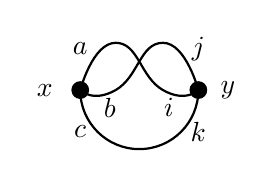
\begin{tikzpicture}[scale = 1.5, baseline=-1mm]
      % lines
      \draw[thick] plot[smooth, tension=1] coordinates { (0, 0) (.3, 0) (.7, .4) (1, 0) };
      \draw[thick] plot[smooth, tension=1] coordinates { (0, 0) (.3, .4) (.7, 0) (1, 0) };
      \draw[thick] (0, 0) arc (-180:0:.5);
      % nodes
      \draw[fill=black] (0, 0) circle (2pt);
      \draw[fill=black] (1, 0) circle (2pt);
      \node at (-.3, 0) {$x$};
      \node at (1.25, 0) {$y$};
      \node at (0, .35) {$a$};
      \node at (.25, -.15) {$b$};
      \node at (0, -.35) {$c$};
      \node at (1, .35) {$j$};
      \node at (0.75, -.15) {$i$};
      \node at (1, -.35) {$k$};
    \end{tikzpicture}
  \end{equation*}
  but no such graph isomorphism exists for between the following graphs.
  \begin{equation*}
  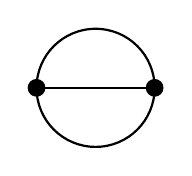
\begin{tikzpicture}[scale = 1.5, baseline=-1mm]
    % lines
    \draw[thick] (0, 0) -- (1, 0);
    \draw[thick] (0, 0) arc (180:0:.5);
    \draw[thick] (0, 0) arc (-180:0:.5);
    % nodes
    \draw[fill=black] (0, 0) circle (2pt);
    \draw[fill=black] (1, 0) circle (2pt);
  \end{tikzpicture}
  \qquad \ncong \qquad
  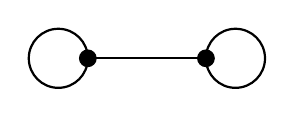
\begin{tikzpicture}[scale =1.5, baseline=-1mm]
    % lines
    \draw[thick] (0, 0) -- (1, 0);
    \draw[thick] (-.25, 0) circle (2.5mm);
    \draw[thick] (1.25, 0) circle (2.5mm);
    % nodes
    \draw[fill=black] (0, 0) circle (2pt);
    \draw[fill=black] (1, 0) circle (2pt);
  \end{tikzpicture}
  \end{equation*}
\end{example}

\begin{example}
  Consider homogeneous polynomials $P_d \in \Sym^d V^\vee$. We compute
  \begin{equation*}
    \bigavg{P_0(x)^{V_0} \dots P_D(x)^{V_D}}
    = \sum_{[\sigma]} \frac{|G|}{|\Aut \Gamma_\sigma|}
    (Q^{-1})^{\otimes m} \circ \sigma \circ (P_0^{V_0} \otimes \dots \otimes P_D^{V_D}) 
  \end{equation*}
  where
  \begin{equation*}
    |G| = \prod_{d = 0}^D (d!)^{V_d} V_d!.
  \end{equation*}
  We can rewrite this as
  \begin{equation*}
    \bigavg{P_0(x)^{V_0} \dots P_D(x)^{V_D}}
    = \biggl( \prod_{d = 0}^D (d!)^{V_d} V_d! \biggr)
    \sum_{\Gamma} \frac{1}{|\Aut \Gamma|} \Phi_{Q^{-1}, \{P_d\}} (\Gamma)
  \end{equation*}
  where we relabel the sum as being over graphs, to which we apply the following procedure.
  \begin{equation*}
    \begin{tikzcd}[sep=small]
    & \Phi_{Q^{-1}, \{{P_d}\}_{d = 0}^D} (\Gamma) \arrow[dr] \arrow[dl] & \\
      \text{label vertices } P_d \arrow[dr] & & \text{label edges } Q^{-1} \arrow[dl] \\
    & \text{contract} &
  \end{tikzcd}
  \end{equation*}
\end{example}

\begin{example}
  For $\Psi \in \Sym^2 V^\vee$ we check that
  \begin{equation*}
    \bigavg{\Psi^3}
    = 8 \cdot 3! \biggl(
      \frac{1}{8 \cdot 3!} \hspace{-4mm}
      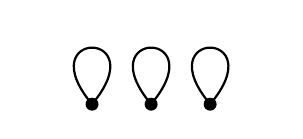
\begin{tikzpicture}[scale=2.5, baseline=2mm]
        % node
        \draw[fill=black] (0, 0) circle (.3mm);
        \draw[fill=black] (.3, 0) circle (.3mm);
        \draw[fill=black] (.6, 0) circle (.3mm);
        % lines
        \draw[thick] (0, 0) to[out=50, in=130, loop] (0, 0);
        \draw[thick] (.3, 0) to[out=50, in=130, loop] (.3, 0);
        \draw[thick] (.6, 0) to[out=50, in=130, loop] (.6, 0);
      \end{tikzpicture}
      \hspace{-4mm} + \frac{1}{8} \hspace{-3mm}
      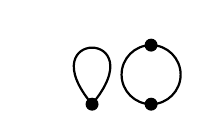
\begin{tikzpicture}[scale=2.5, baseline=2mm]
        % node
        \draw[fill=black] (0, 0) circle (.3mm);
        \draw[fill=black] (.3, 0) circle (.3mm);
        \draw[fill=black] (.3, .3) circle (.3mm);
        % lines
        \draw[thick] (0, 0) to[out=50, in=130, loop] (0, 0);
        \draw[thick] (.3, .15) circle (1.5mm);
      \end{tikzpicture}
      \hspace{1mm} + \frac{1}{6} \hspace{1mm}
      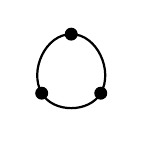
\begin{tikzpicture}[scale=2.5, baseline=2mm]
        % node
        \draw[fill=black] (0, 0) circle (.3mm);
        \draw[fill=black] (.3, 0) circle (.3mm);
        \draw[fill=black] (.15, .3) circle (.3mm);
        % lines
        \draw[thick] (0, 0) to[out=120, in=180] (.15, .3);
        \draw[thick] (.15, .3) to[out=0, in=60] (.3, 0);
        \draw[thick] (0, 0) to[out=-60, in=240] (.3, 0);
      \end{tikzpicture}
    \biggr).
  \end{equation*}
\end{example}

% ── Perturbed Gaussian ────────────────────────────────────────────────
\subsection{Perturbed Gaussian}

We define a \textbf{perturbed} Gaussian integral
\begin{equation*}
  \int_{\Rbb^n}^\text{pert} \drm x \euler^{-\frac{1}{2} Q(x, x) + p(x)}
  = \biggl( \int_{\Rbb^n}^\text{pert} \drm x \euler^{\frac{1}{2} Q(x, x)} \biggr) \bigavg{\euler^{p(x)}}
\end{equation*}
where
\begin{equation*}
  p(x) = \sum_{d = 0}^D \frac{g_d P_d}{d!}, \qquad P_d \in \Sym^d V^\vee.
\end{equation*}

